\subsection{Exercise 26.6}

Sketch the graph of the following functions (Question 1 to 3):

\begin{enumerate}
      \item $f(x)=\dfrac{1}{3} x^3-\dfrac{1}{2} x^2-2 x$
            \sol{}
            \vspace{-1cm}
            \begin{multicols}{2}
                  \begin{flalign*}
                        f(0)                                   & = 0                                                                     & \\
                        \dfrac{1}{3}x^3 - \dfrac{1}{2}x^2 - 2x & = 0                                                                     & \\
                        2x^3 - 3x^2 - 12x                      & = 0                                                                     & \\
                        x(2x^2 - 3x - 12)                      & = 0                                                                     & \\
                        x                                      & = 0 \text{ or } 2x^2 - 3x - 12 = 0                                      & \\
                                                               & = 0 \text{ or } x = \dfrac{3 \pm \sqrt{105}}{4}                           \\
                        f'(x)                                  & = x^2 - x - 2                                                           & \\
                        f''(x)                                 & = 2x - 1                                                                & \\
                        x^2 - x - 2                            & = 0                                                                     & \\
                        (x - 2)(x + 1)                         & = 0                                                                     & \\
                        x                                      & = 2 \text{ or } x = -1                                                  & \\
                        f(2)                                   & = \dfrac{1}{3}\left(2\right)^3 - \dfrac{1}{2}\left(2\right)^2 - 2(2)      \\
                                                               & = \dfrac{8}{3} - 2 - 4                                                    \\
                                                               & = -\dfrac{10}{3}                                                          \\
                        f(-1)                                  & = \dfrac{1}{3}\left(-1\right)^3 - \dfrac{1}{2}\left(-1\right)^2 - 2(-1)   \\
                                                               & = -\dfrac{1}{3} - \dfrac{1}{2} + 2                                        \\
                                                               & = \dfrac{7}{6}                                                            \\
                        f''(2)                                 & = 3 > 0                                                                   \\
                        f''(-1)                                & = -3 < 0
                  \end{flalign*}

                  \begin{flalign*}
                        2x - 1                     & = 0                                                                                                              & \\
                        x                          & = \dfrac{1}{2}                                                                                                   & \\
                        f\left(\dfrac{1}{2}\right) & = \dfrac{1}{3}\left(\dfrac{1}{2}\right)^3 - \dfrac{1}{2}\left(\dfrac{1}{2}\right)^2 - 2\left(\dfrac{1}{2}\right)   \\
                                                   & = \dfrac{1}{24} - \dfrac{1}{8} - 1                                                                                 \\
                                                   & = -\dfrac{13}{12}
                  \end{flalign*}
                  $x$-intercepts: $\left(0, 0\right)$, $\left(\dfrac{3 - \sqrt{105}}{4}, 0\right)$, $\left(\dfrac{3 + \sqrt{105}}{4}, 0\right)$

                  \noindent $y$-intercept: $(0, 0)$

                  \noindent Relative maximum: $\left(-1, \dfrac{7}{6}\right)$

                  \noindent Relative minimum: $\left(2, -\dfrac{10}{3}\right)$

                  \noindent Points of inflection: $\left(\dfrac{1}{2}, -\dfrac{13}{12}\right)$

                  \noindent Convex up: $\left(-\infty, \dfrac{1}{2}\right)$

                  \noindent Convex down: $\left(\dfrac{1}{2}, \infty\right)$
            \end{multicols}
            \vfill\null
            \begin{center}
                  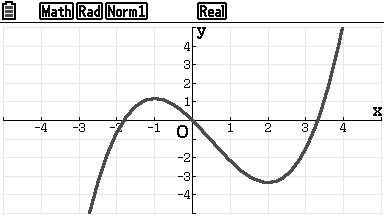
\includegraphics[scale=0.7]{26-graph2.png}
            \end{center}
            \vfill\null
            \newpage

      \item $f(x)=x^4-32 x+10$
            \sol{}
            \vspace{-0.6cm}
            \begin{vwcol}[widths={0.3,0.7},justify=flush,rule=0pt,indent=1em]
                  \begin{flalign*}
                        f(0)      & = 10               & \\
                        f'(x)     & = 4x^3 - 32        & \\
                        f''(x)    & = 12x^2            & \\
                        4x^3 - 32 & = 0                & \\
                        x         & = 2                & \\
                        f(2)      & = 2^4 - 32(2) + 10   \\
                                  & = -38              & \\
                        f''(2)    & = 48 > 0           & \\
                        12x^2     & = 0                & \\
                        x         & = 0                & \\
                        f(0)      & = 10
                  \end{flalign*}
                  y-intercept: $(0, 10)$

                  \noindent Relative minimum: $(2, -38)$

                  \noindent Points of inflection: $(0, 10)$

                  \noindent Convex down: $(-\infty, \infty)$
                  \newpage
                  \vspace*{2cm}
                  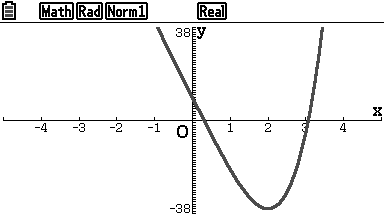
\includegraphics[scale=0.7]{26-graph3.png}
            \end{vwcol}

      \item $f(x)=(x-1)^3(x-2)$
            \sol{}
            \vspace{-1cm}
            \begin{multicols}{2}
                  \begin{flalign*}
                        f(0)                         & = 2                                                     & \\
                        (x-1)^3(x-2)                 & = 0                                                       \\
                        x                            & = 1 \text{ or } x = 2                                     \\
                        f'(x)                        & = 3(x-1)^2(x-2) + (x-1)^3                                 \\
                                                     & = (x-1)^2(3x-6+x-1)                                       \\
                                                     & = (x-1)^2(4x-7)                                           \\
                        f''(x)                       & = 2(x-1)(4x-7) + (x-1)^2(4)                               \\
                                                     & = 2(x-1)(4x-7+2x-2)                                       \\
                                                     & = 2(x-1)(6x-9)                                            \\
                                                     & = 6(x-1)(2x-3)                                            \\
                        (x-1)^2(4x-7)                & = 0                                                       \\
                        x                            & = 1 \text{ or } x = \dfrac{7}{4}                          \\
                        f(1)                         & = 0                                                       \\
                        f\left(\dfrac{7}{4}\right)   & = \left(\dfrac{3}{4}\right)^3\left(-\dfrac{1}{4}\right)   \\
                                                     & = -\dfrac{27}{256}                                        \\
                        f''(1)                       & = 0                                                       \\
                        f''\left(\dfrac{7}{4}\right) & = 6\left(\dfrac{3}{4}\right)\left(\dfrac{7}{2}-3\right)   \\
                                                     & = \dfrac{9}{4} > 0                                      &
                  \end{flalign*}

                  \begin{flalign*}
                        6(x-1)(2x-3)               & = 0                                                     \\
                        x                          & = 1 \text{ or } x = \dfrac{3}{2}                        \\
                        f(1)                       & = 0                                                     \\
                        f\left(\dfrac{3}{2}\right) & = \left(\dfrac{1}{2}\right)^3\left(-\dfrac{1}{2}\right) \\
                                                   & = -\dfrac{1}{16}
                  \end{flalign*}
                  $x$-intercepts: $(1, 0)$, $\left(2, 0\right)$

                  \noindent $y$-intercept: $(0, 2)$

                  \noindent Relative minimum: $\left(\dfrac{7}{4}, -\dfrac{27}{256}\right)$

                  \noindent Points of inflection: $\left(1, 0\right)$, $\left(\dfrac{3}{2}, -\dfrac{1}{16}\right)$

                  \noindent Convex downwards: $\left(-\infty, 1\right)$, $\left(\dfrac{3}{2}, \infty\right)$

                  \noindent Convex upwards: $\left(1, \dfrac{3}{2}\right)$
            \end{multicols}
            \begin{center}
                  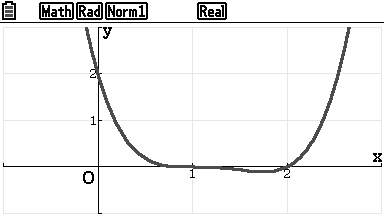
\includegraphics[scale=0.6]{26-graph4.png}
            \end{center}

      \item Given the function $f(x) = x^3(4-x)$.
            \begin{enumerate}
                  \begin{multicols}{2}
                        \item Find the extreme values and the intervals of increasing and decreasing of
                        $f(x)$. \sol{}
                        \begin{flalign*}
                              f(x)        & = 4x^3 - x^4      \\
                              f'(x)       & = 12x^2 - 4x^3    \\
                                          & = 4x^2(3 - x)     \\
                              4x^2(3 - x) & = 0               \\
                              x = 0       & \text{ or } x = 3 \\
                              f(0)        & = 0               \\
                              f(3)        & = 27              \\
                              f''(x)      & = 24x - 12x^2     \\
                              f''(0)      & = 0               \\
                              f''(3)      & = 36 > 0
                        \end{flalign*}
                        $\therefore$ Relative maximum: $f(3) = 27$

                        In the interval $(-\infty, 0)$, $f'(x) > 0$, so $f(x)$ is increasing in the
                        interval $(-\infty, 0]$.

                        In the interval $(0, 3)$, $f'(x) > 0$, so $f(x)$ is increasing in the interval
                        $[0, 3]$.

                        In the interval $(3, \infty)$, $f(x)$ is decreasing in the interval $[3,
                                          \infty)$. \columnbreak

                                                \item Find the points of inflection and the intervals of convexity and concavity of
                                          $f(x)$. \sol{}
                                                \begin{flalign*}
                                                      24x - 12x^2 & = 0               \\
                                                      x(2 - x)    & = 0               \\
                                                      x = 0       & \text{ or } x = 2 \\
                                                      f(0)        & = 0               \\
                                                      f(2)        & = 16
                                                \end{flalign*}
                                          $\therefore$ Point of inflection: $(2, 16)$, $(0, 0)$

                                                In the interval $(-\infty, 0)$, $f''(x) < 0$, so $f(x)$ is convex upward in the
                                                interval $(-\infty, 0]$.

                        In the interval $(0, 2)$, $f''(x) < 0$, so $f(x)$ is convex upward in the
                        interval $[0, 2]$.

                        In the interval $(2, \infty)$, $f''(x) > 0$, so $f(x)$ is convex downward in
                        the interval $[2, \infty)$.
                  \end{multicols}

                  \item Hence, sketch the graph of $f(x)$. \sol{}
                        \begin{center}
                              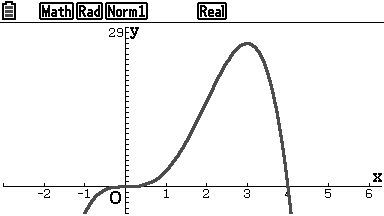
\includegraphics[scale=0.6]{26-graph5.png}
                        \end{center}
            \end{enumerate}
\end{enumerate}